\documentclass[a4paper,12pt]{article}
\usepackage{graphicx}
\usepackage[a4paper,margin=1in]{geometry}
\usepackage{titlesec}
\usepackage{hyperref}
\usepackage{amsmath}    % For math environments and symbols
\usepackage{amssymb}    % For \mathbb and other math symbols
\usepackage{amsfonts}   % Additional math fonts
\usepackage{float}
\setlength{\abovecaptionskip}{-2pt}  
\setlength{\belowcaptionskip}{1pt}
\usepackage{subcaption}
\usepackage[numbers]{natbib}


% Title format
\titleformat{\section}{\large\bfseries}{\thesection}{1em}{}

% Title settings
\title{
    \includegraphics[scale=0.4]{Cam_logo_bw.png}\\
    \vspace{0.5cm}
    M2 Deep Learning - Coursework Assignment
}
\author{Raunaq Rai (rsr45@cam.ac.uk)\\
    Data Intensive Science, Department of Physics, University of Cambridge
}
\date{04 April, 2025 \\ \vspace{0.2cm} {\small Word Count: XXX}}

\begin{document}

\maketitle

\section*{Introduction}

Large Language Models (LLMs) have revolutionised natural language processing and have recently shown promise in domains beyond text, including time-series forecasting \citep{gruver2023language}. In this coursework, we explore the application of LoRA (Low-Rank Adaptation) \citep{hu2021lora} to the Qwen2.5-Instruct model \citep{qwen2.5}, a transformer-based LLM, for forecasting predator-prey population dynamics as described by the Lotka–Volterra equations.

Building on the methodology proposed in the LLMTIME framework \citep{gruver2023language}, which adapts numeric sequences into a tokenizer-friendly format, we examine how Qwen2.5-Instruct can be repurposed for numerical prediction tasks. The objective is to fine-tune the model on a dataset of simulated predator-prey trajectories using LoRA, a parameter-efficient method that allows adaptation of pretrained models without updating all weights.

Our experiments are conducted under strict computational constraints, with a maximum allowable budget of $10^{17}$ floating point operations (FLOPS), encouraging efficient training practices. The provided dataset consists of 1,000 synthetic time series representing prey and predator population dynamics, formatted as 100 time steps per sequence with two variables per step.

This report outlines the implementation of LLMTIME preprocessing, baseline evaluation of the untrained model, LoRA fine-tuning with hyperparameter sweeps, and analysis of forecasting performance under compute-efficient constraints. Our findings highlight the potential of adapting LLMs for scientific time-series forecasting and provide recommendations for future work in compute-constrained settings.

\section{Compute Constraint}

This coursework promotes efficient experimentation under a strict compute budget of $10^{17}$ floating point operations (FLOPs) across all reported experiments. This constraint mirrors real-world limitations and encourages careful model design and evaluation, particularly in environments where access to large-scale compute is restricted. Under ideal utilisation, this budget equates to approximately five hours of GPU processing time on a MacBook M1 Pro.

\subsection*{FLOP Accounting Principles}

FLOP costs are calculated using simplified, hardware-agnostic assumptions. Table~\ref{tab:flops_primitives} provides the per-operation FLOP estimates. For instance, multiplying an $m \times n$ matrix by an $n \times p$ matrix requires:
\begin{equation}
\text{FLOPs}_{\text{matmul}} = m \times p \times (2n - 1)
\end{equation}
We assume backpropagation incurs double the cost of the forward pass, yielding:
\begin{equation}
\text{FLOPs}_{\text{train}} = 3 \times \text{FLOPs}_{\text{forward}}
\end{equation}

\begin{table}[h]
  \centering
  \caption{FLOPs Accounting for Primitive Operations}
  \label{tab:flops_primitives}
  \begin{tabular}{lc}
    \hline
    Operation & FLOPs \\
    \hline
    Addition / Subtraction / Negation (float or int) & 1 \\
    Multiplication / Division / Inverse (float or int) & 1 \\
    ReLU / Absolute Value & 1 \\
    Exponentiation / Logarithm & 10 \\
    Sine / Cosine / Square Root & 10 \\
    \hline
  \end{tabular}
\end{table}

\subsection*{FLOP Estimator Implementation}

To systematically estimate the computational cost of each experiment, we implemented a modular FLOP estimator in Python. This estimator models a forward pass through the Qwen2.5-0.5B architecture at the operation level, breaking down FLOPs into five categories: additions, multiplications, divisions, exponentiations, and square roots.

The estimator accounts for every trainable and non-trainable component of the model. For a given sequence length $n$, the estimator computes the total number of FLOPs for each of the following:

\begin{itemize}
  \item \textbf{Token Embeddings:} These are retrieved via indexing and incur no arithmetic FLOPs.
  
  \item \textbf{Positional Embeddings:} Sinusoidal encodings are added to token embeddings: $n \times d_{\text{model}}$ additions.

  \item \textbf{Multi-head Attention (per layer):}
  \begin{itemize}
    \item \textit{Query, Key, Value projections:} Linear transformations to $d_{\text{head}}$ per head; includes multiplications and bias additions.
    \item \textit{Dot-product attention:} Computation of $QK^T$, scaling, softmax, and weighted sum with $V$.
    \item \textit{Softmax:} Includes exponentiations, summation, and division.
    \item \textit{Output projection:} Concatenation of heads followed by linear transformation.
  \end{itemize}

  \item \textbf{Feedforward MLP (with SwiGLU) \citep{shazeer2020glu}:}
  \begin{itemize}
    \item Two parallel up-projections (gated MLP) and a down-projection.
    \item SwiGLU activation, combining SiLU and elementwise multiplication, is approximated as 22 FLOPs per hidden unit.
  \end{itemize}

  \item \textbf{RMSNorm Layers \citep{zhang2019root}:}
  \begin{itemize}
    \item Elementwise squaring, summation, root, division, and scaling by learned $\gamma$.
  \end{itemize}

  \item \textbf{LoRA Projections (if used) \citep{hu2021lora}:}
  \begin{itemize}
    \item Low-rank down and up-projections added to the frozen weights.
    \item Includes multiplications, additions, and an elementwise residual connection.
  \end{itemize}

  \item \textbf{Final Projection:}
  \begin{itemize}
    \item Linear layer projecting to vocabulary logits: $n \times d_{\text{model}} \times V$ multiplications and additions.
  \end{itemize}
\end{itemize}

These per-layer estimates are summed across all 24 transformer blocks, and added to the overhead of input/output layers. FLOPs for different sequence lengths, LoRA ranks, and model dimensions are configurable through function arguments, enabling detailed accounting for any experimental configuration.

\subsection*{Estimating Backward Pass Cost}

The exact computation of FLOPs for backpropagation is non-trivial and implementation-specific. In practice, the backward pass includes:

\begin{itemize}
  \item Derivatives for every parameter (including gradients for each tensor)
  \item Multiplications and additions for each chain rule application
  \item Memory reuse optimisations depending on the framework
\end{itemize}

For the purposes of this coursework, we assume that the backward pass is approximately double the cost of the forward pass. This is a conservative estimate, as it does not account for optimisations such as gradient checkpointing or memory reuse.

\begin{itemize}
  \item Each forward operation has a corresponding gradient computation (typically with similar or higher cost).
  \item Additional operations such as gradient accumulation, weight updates (e.g. for LoRA), and some recomputation of activations.
\end{itemize}

Thus, the total training FLOPs are given by:
\begin{equation}
\text{FLOPs}_{\text{train}} = \text{FLOPs}_{\text{forward}} + \text{FLOPs}_{\text{backward}} + \text{FLOPs}_{\text{update}} \approx 3 \times \text{FLOPs}_{\text{forward}}
\end{equation}


\section{Baseline: LLMTIME Preprocessing Implementation}

The first task was to implement the LLMTIME preprocessing scheme \citep{gruver2023language} to convert multivariate time-series data into a format suitable for Qwen2.5-Instruct. This was done by creating a dedicated Python module \texttt{src/preprocessor.py} containing a class \texttt{LLMTIMEPreprocessor}, which formats and tokenizes time-series data according to the scheme described in the coursework.

\subsection*{Scaling and Formatting}

Each sample consists of a pair of sequences: prey and predator population values over time. These values often differ significantly in scale, both between and within samples, which can lead to inconsistencies in token length and hinder model generalisation if left unprocessed.

To address this, a per-sample scaling factor $\alpha$ is computed to normalise the numerical range. Specifically, $\alpha$ is chosen as:
\begin{equation}
\alpha = \max\left(\text{percentile}_{95}(\text{prey}),\ \text{percentile}_{95}(\text{predator})\right) / 10
\end{equation}
This dynamic, data-dependent approach ensures that most values fall within a range of approximately $[0, 10]$, regardless of the absolute scale of the original input. By avoiding fixed global scaling, the model remains robust to distributional shifts across samples.

Each value is then scaled by $\alpha$ and rounded to a fixed number of decimal places (default: two). This rounding ensures token consistency and limits the number of unique tokens generated by the tokenizer, improving model efficiency and reducing overfitting to numeric noise.

\subsection*{LLMTIME Encoding}

Following the LLMTIME convention, each timestep is represented as a pair of variables (prey, predator), separated by a comma. Consecutive timesteps are separated by a semicolon. This ensures clarity for tokenization and decoding. For example, a sequence of three timesteps would be formatted as:
\begin{center}
\texttt{0.25,1.50;0.27,1.47;0.31,1.42}
\end{center}

While the original LLMTIME implementation by \citet{gruver2023language} removes decimal points to reduce sequence length—especially for GPT-style models that tokenize numbers into subword units—we retain the decimal point in our implementation for several important reasons:

\begin{itemize}
  \item Qwen2.5's tokenizer already tokenizes numeric strings into digit-level tokens without requiring digit spacing or decimal removal.
  \item Removing the decimal point would introduce additional digits and increase sequence length without benefit.
  \item Preserving the decimal enhances human interpretability and simplifies decoding during inference.
  \item The coursework specification explicitly recommends retaining the decimal point and avoiding space-separated digit encoding.
\end{itemize}

\subsection*{Tokenization}

Once formatted, the numeric string is passed through Qwen2.5’s tokenizer using Hugging Face’s \texttt{AutoTokenizer} interface. Each digit and punctuation mark is tokenized into its own token. For example:
\begin{verbatim}
tokenizer("1.23", return_tensors="pt")["input_ids"].tolist()[0]
\end{verbatim}
yields:
\begin{verbatim}
[16, 13, 17, 18]
\end{verbatim}
confirming tokenization into digit and punctuation tokens.

\subsection*{Example Sequences and Tokenization}

We illustrate the LLMTIME preprocessing pipeline with two example predator-prey sequences. For each, we show:

\begin{itemize}
  \item the original prey and predator population values (first 5 timesteps),
  \item the scaled and formatted text string,
  \item the tokenized output (Qwen2.5 input IDs),
  \item the computed scale factor $\alpha$.
\end{itemize}

\paragraph{Example 1.}
\begin{itemize}
  \item \textbf{Original Input:}
  \begin{verbatim}
Prey:     [2.9, 3.2, 3.8, 4.5, 5.1]
Predator: [1.1, 0.9, 0.7, 0.6, 0.5]
  \end{verbatim}

  \item \textbf{Scale Factor $\alpha$:}
  \begin{verbatim}
0.498
  \end{verbatim}


  \item \textbf{Formatted Sequence:}
  \begin{verbatim}
5.82,2.21;6.43,1.81;7.63,1.41;9.04,1.20;10.24,1.00
  \end{verbatim}

  \item \textbf{Tokenized Output (Qwen2.5 input IDs):}
  \begin{verbatim}
[20, 13, 23, 17, 11, 17, 13, 17, 16, 26, 21, 13, 19, 18, 11,
16, 13, 23, 16, 26, 22, 13, 21, 18, 11, 16, 13, 19, 16, 26,
24, 13, 15, 19, 11, 16, 13, 17, 15, 26, 16, 15, 13, 17, 19,
11, 16, 13, 15, 15]
  \end{verbatim}
\end{itemize}

\paragraph{Example 2.}
\begin{itemize}
  \item \textbf{Original Input:}
  \begin{verbatim}
Prey:     [1.5, 1.8, 2.1, 2.4, 2.7]
Predator: [2.8, 2.5, 2.2, 1.9, 1.6]
  \end{verbatim}

  \item \textbf{Scale Factor $\alpha$:}
  \begin{verbatim}
0.274
  \end{verbatim}


  \item \textbf{Formatted Sequence:}
  \begin{verbatim}
5.47,10.22;6.57,9.12;7.66,8.03;8.76,6.93;9.85,5.84
  \end{verbatim}

  \item \textbf{Tokenized Output (Qwen2.5 input IDs):}
  \begin{verbatim}
[20, 13, 19, 22, 11, 16, 15, 13, 17, 17, 26, 21, 13, 20, 22,
11, 24, 13, 16, 17, 26, 22, 13, 21, 21, 11, 23, 13, 15, 18,
26, 23, 13, 22, 21, 11, 21, 13, 24, 18, 26, 24, 13, 23, 20,
11, 20, 13, 23, 19]
  \end{verbatim}
\end{itemize}

\begin{figure}[ht]
    \centering
    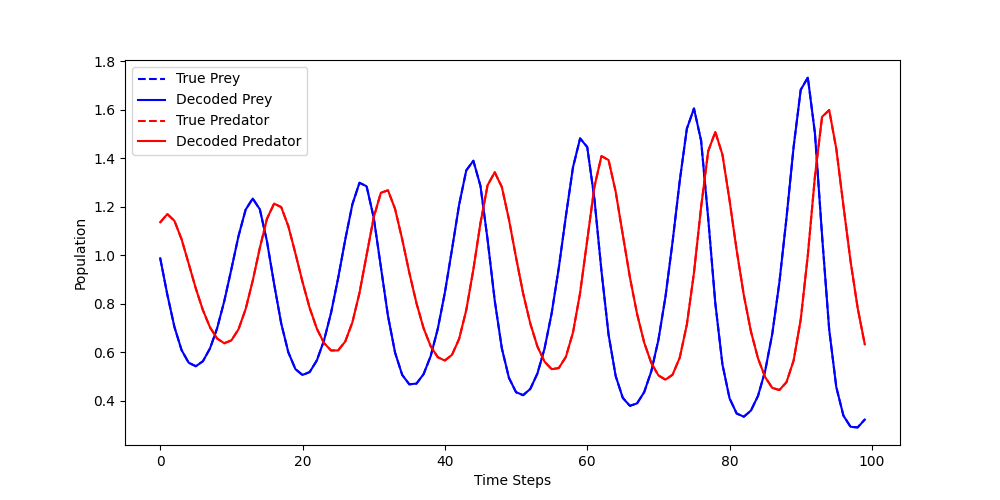
\includegraphics[width=\textwidth]{true_vs_decoded.png}
    \caption{Decoded output vs. ground truth for the 972\textsuperscript{nd} Lotka-Volterra trajectory in the test set. This sequence was passed through the LLMTIME preprocessing pipeline and fed into the untrained Qwen2.5-Instruct model. The resulting output was decoded and rescaled using the same scale factor $\alpha$ applied during encoding. The close alignment between original and decoded values confirms that the preprocessing, tokenization, and decoding pipeline is working as intended.}
    \label{fig:true_vs_decoded}
  \end{figure}
  
  \begin{figure}[ht]
    \centering
    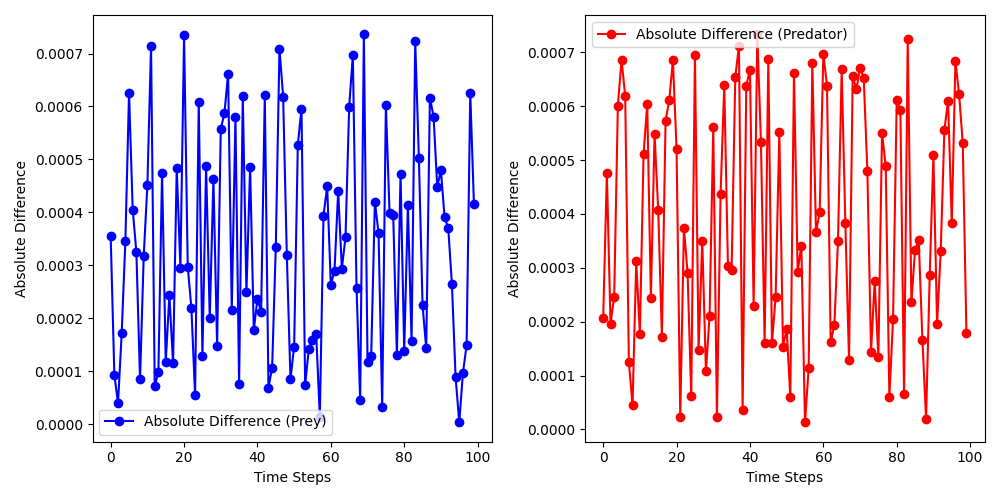
\includegraphics[width=\textwidth]{absolute_differences.png}
    \caption{Absolute differences between true and decoded prey (left) and predator (right) values for the 972\textsuperscript{nd} test sequence. These errors quantify the deviation introduced by the LLMTIME encoding-decoding pipeline. The low magnitude of differences confirms the correctness of the numeric formatting, tokenizer compatibility, and inverse decoding process, independent of model training.}
    \label{fig:absolute_differences}
  \end{figure}
  
  \section{Baseline Evaluation: Forecasting with Untrained Qwen2.5-Instruct}

  We evaluate the zero-shot forecasting capability of the untrained \texttt{Qwen2.5-0.5B-Instruct} model using one example from the dataset (Sample ID 972). The first 50 timesteps are provided as input, and the model is tasked with generating predictions for the remaining 50 steps using the LLMTIME token format.
  
  \subsection*{Language Model Generation and Forward Pass Estimation}
  
  Generation is performed using the Hugging Face \texttt{generate()} API, which operates autoregressively—predicting one token at a time, where each new token requires a full forward pass over the model. The input sequence is constructed from 50 timesteps (each a prey-predator pair), formatted as \texttt{5.38,1.44;...}. In our run, this input tokenized to \textbf{499 tokens}.
  
  To generate 50 new timesteps, we first call \texttt{generate(..., max\_new\_tokens=500)}. Because each timestep typically requires around 10 tokens, this initial attempt may not reach the desired 50-step output. To monitor progress, we count the number of semicolon-separated pairs in the output after each block of generation. If fewer than 100 semicolons (original + generated) are found, we call \texttt{generate(..., max\_new\_tokens=20)} repeatedly until the desired length is reached or we hit a limit.
  
  In this particular run, the model generated a total of \textbf{520 new tokens} to complete 100 timesteps. Since each new token corresponds to one forward pass (under causal decoding), this implies \textbf{520 forward passes} were performed on top of the original 499-token input context.
  
  \textbf{FLOPs Estimation:} To estimate computational cost, we use the Qwen2.5 architecture’s FLOP profile via the \texttt{forwards\_pass\_flops()} utility. Based on our input length of 499 tokens, the model uses approximately \textbf{5.48e11 FLOPs per token} during inference. Therefore, generating 520 tokens requires:
  
  \begin{align*}
  \text{FLOPs} &= 520 \times 5.48 \times 10^{11} = \textbf{2.85} \times 10^{14}
  \end{align*}
  
  This estimate assumes a compute efficiency of 1 and does not account for memory bandwidth, activation caching, or I/O overhead.
  
  \subsection*{Forecasting Performance}
  
  We compare the predicted output (post-decoding and re-scaling) to the true population values for Sample ID 972 using standard metrics:
  
  \begin{itemize}
    \item \textbf{Prey:}
      \begin{itemize}
        \item Mean Squared Error (MSE): 0.1770
        \item Mean Absolute Error (MAE): 0.2485
        \item $R^2$ Score: -0.2812
      \end{itemize}
    \item \textbf{Predator:}
      \begin{itemize}
        \item Mean Squared Error (MSE): 0.2337
        \item Mean Absolute Error (MAE): 0.2793
        \item $R^2$ Score: -1.6260
      \end{itemize}
  \end{itemize}
  
  The prey trajectory shows moderate alignment, albeit with oversmoothing. The predator prediction, however, is unstable, with a negative $R^2$ indicating performance worse than simply predicting the mean. This reflects the model’s lack of understanding of the underlying dynamics without domain-specific training.
  
  \subsection*{Non-Determinism in Generation}
  
  It’s important to note that generation is inherently non-deterministic unless a seed is set. This means different runs on the same input can yield very different outputs—some closer to ground truth, others worse. This behaviour arises from sampling strategies like temperature scaling or nucleus sampling used during decoding.
  
  \subsection*{Compute Assumptions and Efficiency}

  In this coursework, we assume a compute efficiency of 1, meaning all estimated FLOPs are fully utilised during inference without memory or runtime optimisations. Some large-scale language models, such as GPT-4, employ Mixture-of-Experts (MoE) architectures to reduce active parameters per forward pass—this lowers compute cost by activating only a subset of layers during token generation. However, \texttt{Qwen2.5-0.5B-Instruct} does not employ MoE or dynamic routing, meaning that \textbf{all model parameters are active for every forward pass}.
  
  Recent innovations such as SkipDecode~\cite{delcorro2023skipdecode} propose early-exit strategies that skip computation in lower layers during autoregressive decoding. This approach can significantly reduce inference FLOPs while preserving performance, and is compatible with batching and KV cache reuse. Nonetheless, \texttt{Qwen2.5-0.5B-Instruct} does not implement such mechanisms, and so the full model is evaluated on every token without layer skipping or selective computation.
  
  \begin{figure}[h]
      \centering
      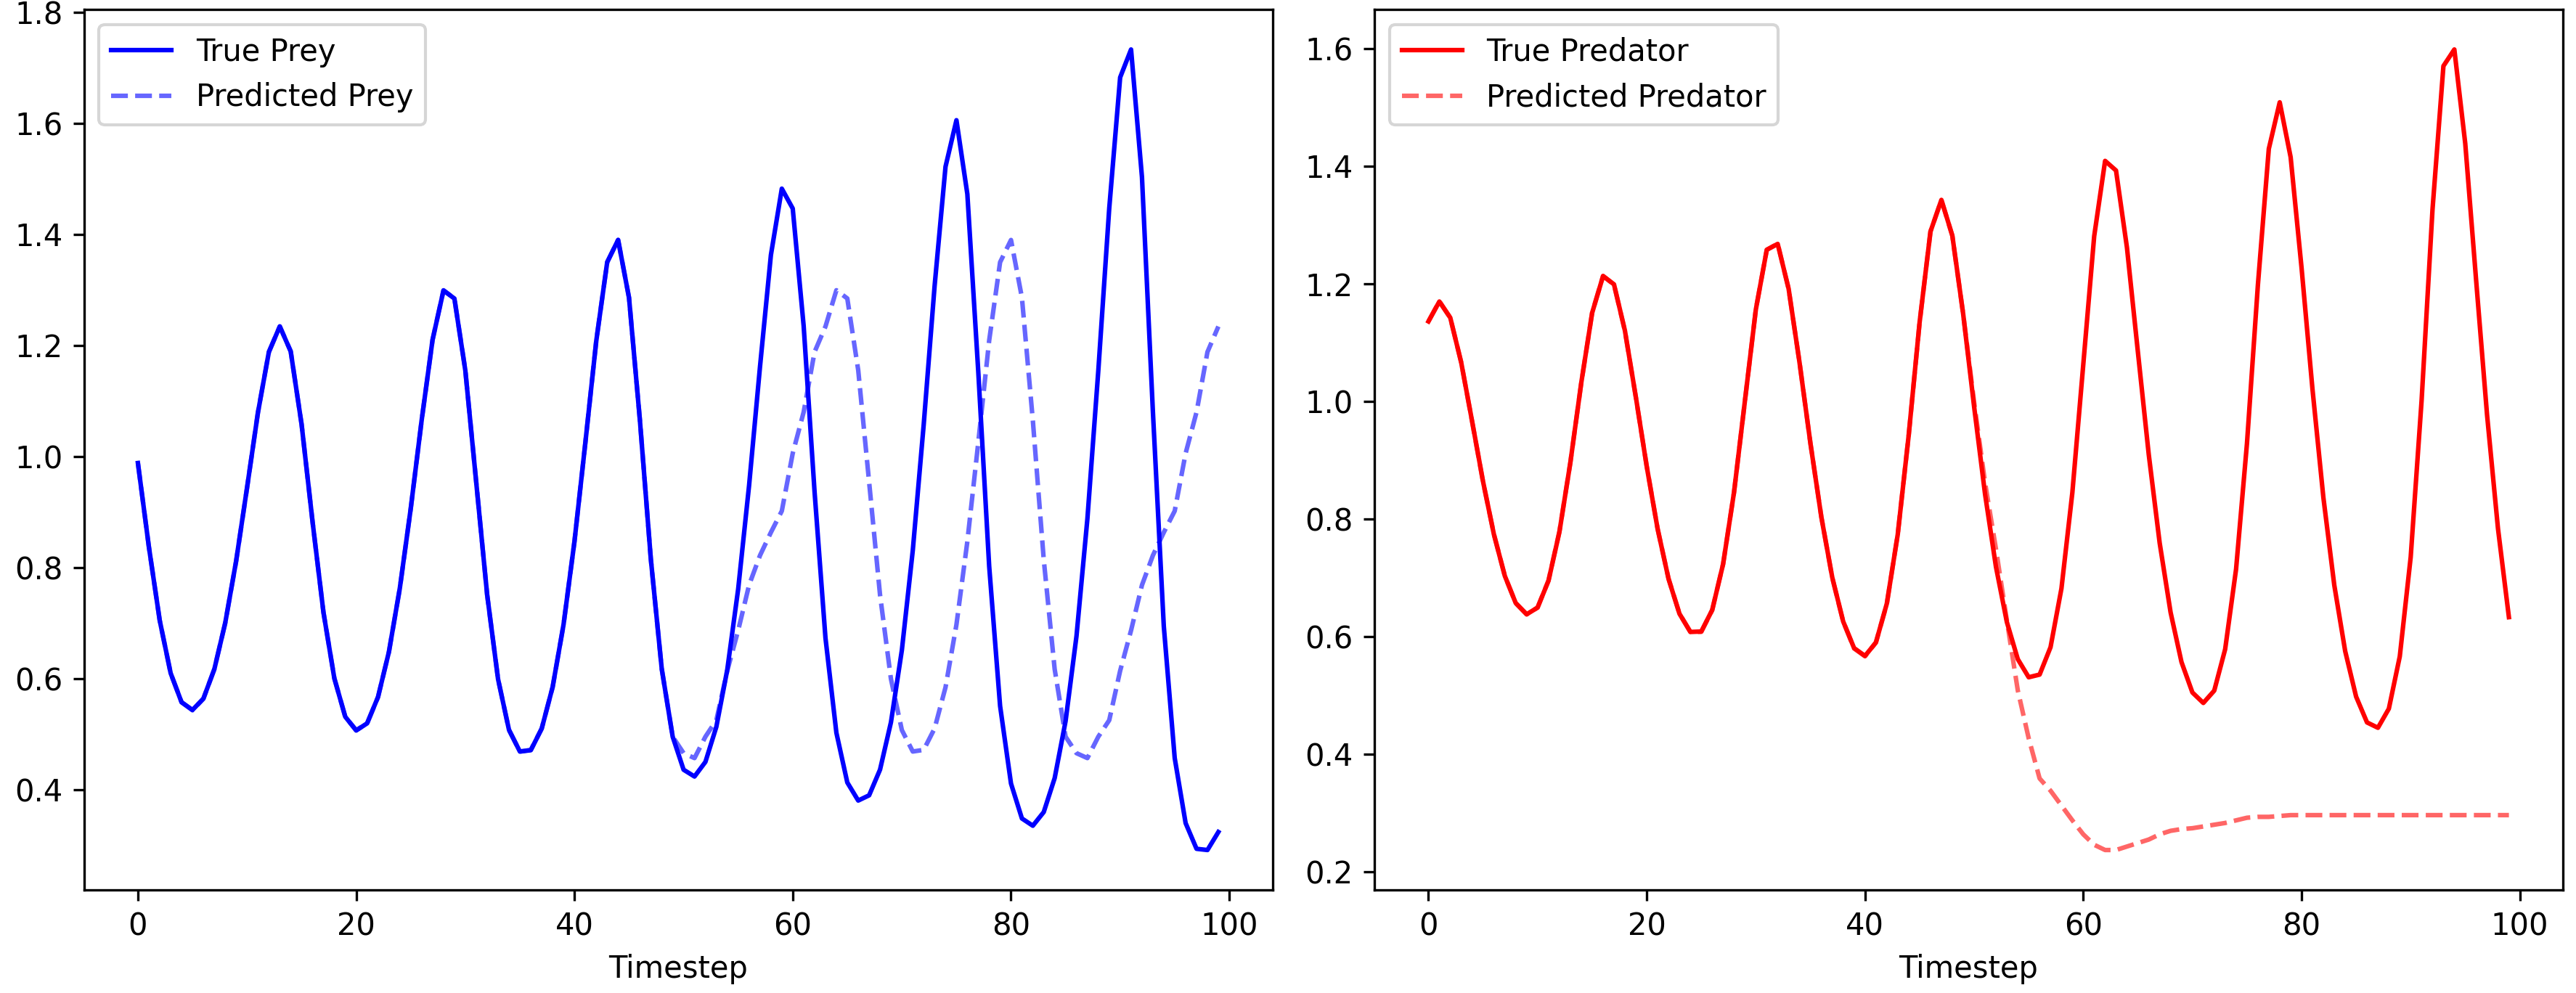
\includegraphics[width=0.9\textwidth]{sample972_untrained.png}
      \caption{Forecasting output of the untrained Qwen2.5-Instruct model on Sample ID 972. The model is prompted with the first 50 timesteps and generates the next 50. Dashed lines show true values; solid lines show decoded predictions.}
      \label{fig:sample972_untrained}
  \end{figure}
  
  The untrained Qwen2.5-Instruct model exhibits some capacity to mimic the structure of the prey trajectory under LLMTIME formatting, likely due to its strong inductive bias and learned text patterns. However, it struggles with the more complex predator dynamics, which results in erratic predictions. This reinforces the need for fine-tuning or domain-specific adaptation when applying language models to structured forecasting problems.
  
  \section{FLOP Accounting for Transformer Components}

  To estimate the total FLOPs consumed by the Qwen2.5-0.5B-Instruct model, we explicitly mapped every major component in the forward pass to primitive arithmetic operations and computed their FLOP costs using the provided FLOPs table (Table~\ref{tab:flops_primitives}). Below we summarise the decomposition of each operation.
  
  \subsection*{Token and Positional Embeddings}
  \begin{itemize}
    \item \textbf{Token Embeddings:} Retrieved via table lookup — \textbf{0 FLOPs}.
    \item \textbf{Positional Embedding Addition:} $n \times d_{\text{model}}$ additions.
  \end{itemize}
  
  \subsection*{RMSNorm (applied before attention, after attention, and before MLP)}
  For each token:
  \begin{itemize}
    \item Square each element: $n \times d$ multiplications.
    \item Sum across dimension: $n \times (d - 1)$ additions.
    \item Square root: $n$ square root operations.
    \item Divide each element by norm: $n \times d$ divisions.
    \item Scale with learned weight: $n \times d$ multiplications.
  \end{itemize}
  \textbf{Total:} $n \times (2d)$ multiplications, $n \times (d - 1)$ additions, $n + n \times d$ divisions, $n$ square roots.
  
  \subsection*{Multi-Head Attention (per layer)}
  Let $h$ be the number of heads and $d_h = d / h$.
  \begin{itemize}
    \item \textbf{Q/K/V Projections:} $3 \times n \times d \times d_h$ multiplications and $(3 \times n \times (d - 1) \times d_h)$ additions.
    \item \textbf{Attention Scores:} $n \times n \times d_h$ multiplications and $n \times n \times (d_h - 1)$ additions.
    \item \textbf{Softmax:} For $n^2$ elements:
      \begin{itemize}
        \item Exponentiation: $n^2$
        \item Summation: $n \times (n - 1)$ additions
        \item Normalisation: $n^2$ divisions
      \end{itemize}
    \item \textbf{Softmax-Value Multiplication:} $n \times n \times d_h$ multiplications and $n \times d_h \times (n - 1)$ additions.
    \item \textbf{Concatenation:} Memory operation — \textbf{0 FLOPs}.
    \item \textbf{Final Output Projection:} $n \times d \times d$ multiplications and $n \times (d - 1) \times d$ additions.
  \end{itemize}
  
  \subsection*{MLP Block with SwiGLU (per layer)}
  Let $d_{\text{ff}}$ be the hidden dimension (e.g., 4864).
  \begin{itemize}
    \item \textbf{Up-Projection and Gating:} $2 \times n \times d \times d_{\text{ff}}$ multiplications and $2 \times n \times (d - 1) \times d_{\text{ff}}$ additions.
    \item \textbf{Down-Projection:} $n \times d_{\text{ff}} \times d$ multiplications and $n \times (d_{\text{ff}} - 1) \times d$ additions.
    \item \textbf{SwiGLU Activation:}
      \begin{itemize}
        \item SiLU requires: 1 exp, 1 div, 2 mul, 1 add per unit.
        \item Total: $n \times d_{\text{ff}}$ exponentiations, divisions, additions, and $2 \times n \times d_{\text{ff}}$ multiplications.
      \end{itemize}
  \end{itemize}
  
  \subsection*{Final Projection to Vocabulary Logits}
  \begin{itemize}
    \item \textbf{Linear Projection:} $n \times d \times V$ multiplications and $n \times (d - 1) \times V$ additions.
  \end{itemize}
  
  \subsection*{LoRA (if enabled)}
  For each adapted projection (Q and V):
  \begin{itemize}
    \item \textbf{Down-projection:} $n \times d \times r$ multiplications and $n \times (d - 1) \times r$ additions.
    \item \textbf{Up-projection:} $n \times r \times d$ multiplications and $n \times (r - 1) \times d$ additions.
    \item \textbf{Scaling + Residual Addition:} $n \times d$ multiplications and additions.
  \end{itemize}
  \textbf{Total for one LoRA adapter:} $2 \times$ (down + up) + residual = $(2 \times n \times d \times r + n \times d)$ mults and similar additions.
  
  \subsection*{Summary}
  Each primitive operation has the following FLOP cost:
  \begin{itemize}
    \item Addition / Subtraction / Negation: \textbf{1}
    \item Multiplication / Division / Inverse: \textbf{1}
    \item ReLU / Absolute Value: \textbf{1}
    \item Exponentiation / Logarithm: \textbf{10}
    \item Square Root / Sine / Cosine: \textbf{10}
  \end{itemize}
  
  Using these constants, the total FLOPs can be calculated with:
  \begin{equation}
  \text{Total FLOPs} = \sum_{i=1}^{n} \left( a_i \cdot 1 + m_i \cdot 1 + d_i \cdot 1 + e_i \cdot 10 + s_i \cdot 10 \right)
  \end{equation}
  where $a_i$, $m_i$, $d_i$, $e_i$, and $s_i$ represent the counts of additions, multiplications, divisions, exponentiations, and square roots respectively for each model component.
  
  The complete implementation of this accounting is automated in our Python function \texttt{forwards\_pass\_flops()}, which accepts parameters such as number of tokens, LoRA rank, and returns per-operation and total FLOPs.
  


\bibliographystyle{unsrtnat}
\bibliography{references}


\end{document}
